\chapter{Quantum computation}
The attempt of this chapter is to synthesize as much as possible the boundless field of quantum computation. Trivializing, quantum computation exploits the properties of quantum mechanics (e.g, superposition and entanglement) to perform computation. 
This means a new set of gates, a new unit of information and a new mathematics instead of Boole's one.
\section{The postulates}
We shall start with a general overview of the basic postulates of quantum mechanics. These postulates provide a connection between the physical world and the mathematical formalism of quantum mechanics upon quantum computation is built on.
\begin{postulate}\label{postulate:1}
Associated to any isolated physical system is a Hilbert space $\mathcal{H}$ known as the \emph{state space} of the
system. The system is completely described by its \emph{state vector} $\ket{\psi(t)}$, which is a unit
vector in the system’s state space.
\end{postulate}
\begin{postulate}
The time-evolution of the state of a closed quantum system is described by a
unitary operator. That is, for any evolution of the closed system there exists
a unitary operator $\widehat{U}(t_2,t_1)$ such that if the initial state of the system is $\ket{\psi(t_1)}$ then
after the evolution the state of the system will be:
\begin{equation*}
    \ket{\psi(t_2)} = \hat{U}(t_2,t_1) \ket{\psi(t_1)} \quad \text{with} \quad \hat{U}^\dagger\hat{U} = \hat{\mathbb{I}}\,.
\end{equation*}
\end{postulate}
\begin{postulate}
Quantum measurements are described by a collection $\{M_m\}$ of
measurement operators. These are operators acting on the state space of the
system being measured. The index $m$ refers to the measurement outcomes that
may occur in the experiment. If the state of the quantum system is $\ket{\psi(t)}$
immediately before the measurement then the probability that result m occurs is given by
\begin{equation*}
    p(m) = \expval{M^\dagger_m M_m}{\psi}
\end{equation*}
and the state of the system after the measurement is
\begin{equation*}
    \frac{M_m\ket{\psi}}{\expval{M^\dagger_m M_m}{\psi}}
\end{equation*}
The measurement operators satisfy the \emph{completeness equation}
\begin{equation*}
    \sum_m M_m^\dagger M_m = \mathbb{I}
\end{equation*}
which express the fact that probabilities sum to one: $\sum_n p(m) = \sum_n \expval{M^\dagger_m M_m}{\psi} = 1$.
\end{postulate}
\begin{postulate}\label{postulate:4}
The state space of a composite physical system is the tensor product
of the state spaces of the component physical systems. If we have systems numbered $1$ through $N$:
\begin{equation*}
   \mathcal{H} = \bigotimes_{i=1}^{N}\,\mathcal{H}_i \quad  \text{and} \quad \text{dim}\mathcal{H} = \prod_{i=1}^N \text{dim}\mathcal{H}_i\,.
\end{equation*}
\end{postulate}
\section{Quantum bit}
The definition of qubit (quantum bit) immediately follow from \hyperref[postulate:1]{postulate 1}:
\begin{defn}
A qubit is a system S whose Hilbert space is two-dimensional (i.e. $\text{dim}\mathcal{H}_S = 2$).
\end{defn}
Because of \hyperref[postulate:1]{postulate 1} and according to the definition of vector space we see that every linear combination of a state vector.
\begin{equation}\label{eq:1}
    \bra{\psi} = a \bra{\alpha} + b \bra{\beta} \quad \bra{\alpha},\bra{\beta} \in \mathcal{H}_\psi \quad a,b \in \mathcal{C} \quad \abs{a}^2 + \abs{b}^2 = 1
\end{equation}
is still part of the state space and it still describes the physics of the system. (There is an only constraint: the state has to be normalized as we will discuss in \ref{sec:measurement}, such a rescaling is possible and will be assumed hereafter.) 

Here lies the main difference between bits and qubits: whereas in classical computation only $0$ and $1$ states are allowed in quantum computation also superposition states are perfectly acceptable. What does a superposition states physically mean? If we measure for example \ref{eq:1} the probability of being in the state $\ket{\alpha}$ is  $\abs{a}^2$ and the probability of being in the state $\ket{\beta}$ is $\abs{b}^2$.

According (again) to the \hyperref[postulate:1]{first postulate} the state of a qubit is a vector in a two-dimensional Hilbert space. Let's define it's basis:
\begin{defn}\label{def:computational-basis}
The orthonormal basis of the two-dimensional Hilbert space describing a qubit is called \emph{computational basis} and it's composed by the states $\ket{0}$ and $\ket{1}$ known as \emph{computational basis states}.
\end{defn}
How is a qubit physically made?
It can be a $1/2$ spin particle, an atomic system whose dynamics is described by two (non degenerate) energy level and so on.
Whatever we choose to be our physical realization of the qubit we have an hermitian operator associated to the the observable chosen. The computational basis then will be composed by the eigenstates of the hermitian operator associated with the observable, those state (whatever the operator is) will be labelled as $\{\ket{0},\ket{1}\}$ according to the \hyperref[def:computational-basis]{definition}.

Let's try, for example, to use $1/2$ spin particle. We know that the hermitian operator associated with spin is $S_z$ or $\hat{\sigma}_z = \frac{2}{\hbar} S_z$ and we are okay with that because it has two eigenstates and two non degenerate eigenvales:
\marginpar{An example of how a qubit can be physically implemented}
\begin{align*}
    &\hat{\sigma}_z \ket{\chi_+} = \ket{\chi_+}  \\
    &\hat{\sigma}_z \ket{\chi_-} = -\ket{\chi_-}
\end{align*}
This eigentates (i.e. the spinors) span a two-dimensional Hilbert space\footnote{Note that this is true in general: every hermitian operator admits eigenstates and those eigenstate form a basis for the Hilbert space where the operator itself is defined \cite[p.100]{Shankar}.} and are then the computational basis.
\subsection{Quantum register}
What if 
\begin{defn}
A quantum register is a system QR  with $\text{dim}\mathcal{H}_{QR} = 2^N$.
\end{defn}
\subsection{Entanglement}
\section{Quantum circuits}
A \emph{quantum circuit} is a set of elementary quantum operations, that is a model for quantum computation in which a computation is a sequence of quantum gates.

The basic blocks of a quantum circuit are quantum channels, single-qubit gates, two-qubit gates and the measurement operation which allow us to retrieve the result of the algorithm implemented in the circuit. We shall analyze each component in the following sections.

It follows from the \hyperref[postulate:2]{second postulate} that the dynamical evolution of the qubit due to the various elements of the circuit (gates and channels) is described by a unitary operator. Let us review some of its proprieties: 
\begin{theorem}\label{theorem:1}
There always exist an operator $\hat{H}$ such that $\hat{U}(t) = e^{-i\hat{H}t/\hbar}$ with $\hat{H} = \hat{H}^\dagger$ the Hamiltonian describing the system. \cite{Shankar}
\end{theorem}

Note that the the Hamiltonian being Hermitian guarantees the unitarity of our operator. After the evolution the norm of the input is conserved (which implies that the state is still valid according to \hyperref[postulate:1]{postulate 1}) since
\begin{theorem}
A unitary operator preserves the inner product.
\end{theorem}
\begin{proof}
\begin{equation*}
    \braket{\hat{U}(t)\psi | \hat{U}(t)\psi} = \braket{ \psi | \hat{U}^\dagger(t)\hat{U}(t) | \psi} = \braket{\psi | \psi}
\end{equation*}
\end{proof}


Thanks to \hyperref[theorem:1]{theorem 1} and \hyperref[postulate:2]{postulate 2} we are able to understand the dynamical evolution of the qubit (or the quantum register) due to each gate (or channel) \graffito{State evolution in the circuit.}
\begin{equation}\label{eq:evolution}
     \ket{Q}_\textup{out} \equiv \hat{U}(\tau) \ket{Q}_\textup{in} = e^{-i\tau\hat{H}_Q/\hbar} \ket{Q}_\textup{in}
\end{equation}
where $\tau$ is the time which is physically necessary for the element of the circuit to complete its action, $H_Q$ is the qubit (or quantum register) Hamiltonian and $\ket{Q}_\textup{in}$, $\ket{Q}_\textup{out}$ are the input and output.
\begin{theorem}
For every element of the circuit (gate or transmission channel) acting as $\ket{Q}_\textup{out} = \hat{U} \ket{Q}_\textup{in}$ there exist $\hat{U}^\dagger$ such that $\ket{Q}_\textup{in} = \hat{U}^\dagger \ket{Q}_\textup{out}$.
\end{theorem}
\begin{proof}
It immediately follows from the unitary of the operator $\hat{U} \hat{U}^\dagger = \hat{\mathbb{I}} \rightarrow \hat{U}^{-1} = \hat{U}^\dagger$
\end{proof}
In other words, every operation executed by the circuit is \emph{reversible} and operation with a different number of inputs and outputs (perfectly acceptable in classical computation, an example in \ref{fig:classical-inverse-gate}) are not possible.
\begin{figure}[htb]
\centering
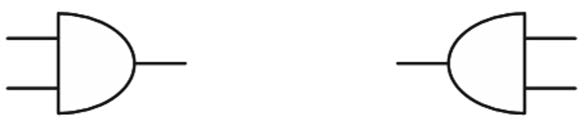
\includegraphics[width=0.3\textwidth]{inverse-gate}
\caption{Classical inverse gate.}
\label{fig:classical-inverse-gate}
\end{figure}
\subsection{Quantum channels}
\begin{figure}[htb]
\[ \Qcircuit {
\lstick{\ket{Q}} & \rstick{\ket{Q}} \qw
}
\]
\caption{Ideal quantum channel.}
\label{fig:quantum-channel}
\end{figure}
A \emph{quantum channel} represents any process that realizes a point-to-point transfer of the quantum information embodied into the state of one qubit $\ket{Q}$. We can picture a quantum channel as a pipeline intended to carry quantum information. We are going to describe memoryless quantum channels (i.e. the output of a channel at a given time depends only upon the corresponding input and not any previous ones).
A quantum channel should not alter the information but just transmit it, thus, from \eqref{eq:evolution}:
\begin{defn}
A \emph{quantum channel} is an evolution operator with $\hat{H}=\hat{\mathbb{I}}$.
\end{defn}
The evolution due to the quantum channel can be readily built:
\begin{equation}\label{eq:quantum-channel}
    \ket{Q}_\textup{out} = \hat{U}(\tau_\textup{ch}) \ket{Q}_\textup{in} = e^{-i\tau_\textup{ch}\hat{\mathbb{I}}} \ket{Q}_\textup{in} = e^{-i\tau_\textup{ch}/\hbar} \ket{Q}_\textup{in}
\end{equation}
as a phase factor does not change the state of the qubit.\footnote{$\ket{\psi'}= \ket{\psi}e^{i\phi}$ since the probability of measuring a specific eigenvalue $\omega$ does not change: $p'(\omega) = \bra{\psi e^{-i\phi}}\mathbb{P}_\omega\ket{\psi e^{i\phi}} = \braket{\psi|\mathbb{P}_\omega|\psi} = p(\omega) \quad \forall \omega\,.$}

Such condition can be obtained in two ways:
\begin{description}
\item[Flying qubit] When the object embodying the qubit can physically move. Its repositioning should be shielded enough to avoid any interaction that could result in $\hat{H} \neq \hat{\mathbb{I}}$.
\item[Still qubit] If the object embodying the qubit cannot move an auxiliary medium is necessary, with the interaction in the medium properly designed so as to guarantee that condition \eqref{eq:quantum-channel} be fulfilled.
\end{description}

\subsection{Single-qubit gates}
Quantum gates are not meant to only transport information like quantum channels, their dynamical evolution is supposed to alter the state.
Single-qubit gates $G_1$ perform an operation on one single qubit. $G_1$ represents the dynamical evolution of the qubit and can therefore be realized by properly designing an Hamiltonian according to \eqref{eq:evolution}:
\begin{equation*}
   \ket{Q}_\textup{out} = G_1\ket{Q}_\textup{in} = e^{-i\hat{H}_Q \tau_{G_1}/\hbar}\ket{Q}_\textup{in}\,.
\end{equation*}

\begin{figure}[htb]
\[ \Qcircuit {
     \lstick{\ket{Q}_\textup{in}}  & \gate{G_1} & \rstick{\ket{Q}_\textup{out}} \qw 
}\]
\caption{One-qubit gate}
\label{fig:one-qubit-gate}
\end{figure}


Once a computational basis has been chosen we can indicate the corresponding matrix representation for the basis vectors as the following
\begin{equation}\label{eq:basis-matrix}
    \ket{0} \rightarrow \begin{pmatrix} 1 \\ 0 \end{pmatrix} \quad \ket{1} \rightarrow \begin{pmatrix} 0 \\ 1 \end{pmatrix}\,.
\end{equation}

Among the most important gates there are \emph{Pauli X gate} and \emph{Pauli Z gate}, their matrix representation according to \ref{eq:basis-matrix} is\footnote{Their matrix representation equals Pauli matrices, hence the name.}
\begin{align*}
    X = 
    \begin{bmatrix}
    0 & 1\\
    1 & 0
    \end{bmatrix} 
    \quad &
     Z = 
    \begin{bmatrix}
    1 & 0\\
    0 & -1
    \end{bmatrix}\,.
\end{align*}
The Pauli-X gate is the quantum equivalent of the NOT gate for classical computers. 
The Pauli-Z gate leaves the basis state $\ket{0}$  unchanged and maps $\ket{1}$  to $-\ket{1}$. Due to this nature, it is sometimes called phase-flip. 
\subsubsection{Hadamard gate}
Finally the \emph{Hadamard gate}. The matrix representation is the following:
\begin{equation}\label{eq:hadamard-gate}
    H = \frac{1}{\sqrt{2}}
    \begin{bmatrix}
    1 & 1\\
    1 & -1
    \end{bmatrix}
\end{equation}
Therefore from \eqref{eq:basis-matrix} we have the action of the gate on the basis states (and using a linear combination of those the action on any qubit):
\begin{equation}
\left\{
\begin{aligned}
    H\ket{0} &= \frac{\ket{0} + \ket{1}}{\sqrt{2}} \\
    H\ket{1} &= \frac{\ket{0} - \ket{1}}{\sqrt{2}}
\end{aligned}
\right.
\end{equation}
This gate is fundamental as it creates a superposition state (i.e. a measurement will have equal probabilities to result in $\ket{1}$ or $\ket{0}$) therefore is often the first step of quantum algorithms as we are going to see in \ref{sec:the-algorithm}.


Let us take an example of a possible physical implementation. Suppose the qubit being implemented by a $1/2$ spin particle according to \eqref{eq:spin-particle}. \graffito{Hadamard gate realized trough a spin particle interacting in a magnetic field.} If the particle interact with a magnetic field $\mathbf{B} = B\mathbf{n}$ with $\mathbf{n} = (\frac{1}{\sqrt{2}}, 0, \frac{1}{\sqrt{2}})$ the Hamiltonian representing the interaction is
\begin{equation*}
    \hat{H} = g\mu_B \mathbf{B} \cdot \hat{\mathbf{S}} = \frac{gB\mu_B}{2} \mathbf{n} \cdot \hat{\boldsymbol{\sigma}} = h \mathbf{n} \cdot \hat{\boldsymbol{\sigma}} \quad \text{with} \quad h \equiv \frac{gB\mu_B}{2}
\end{equation*}
where $\hat{\mathbf{S}} = (\hat{S}^x, \hat{S}^y, \hat{S}^z)$ is the spin operator, $\hat{\boldsymbol{\sigma}} = (\hat{\sigma}^x, \hat{\sigma}^y, \hat{\sigma}^z)$ is the Pauli vector, g is the g-factor and $\mu_B$ is the Bohr magneton.

We know that
\begin{theorem}
\begin{equation*}
e^{i\hat{\boldsymbol{\sigma}} \cdot \mathbf{n}\theta} = \hat{\mathbb{I}}\cos\theta + i\hat{\boldsymbol{\sigma}} \cdot \mathbf{n} \sin\theta
\end{equation*}
\end{theorem}
\begin{proof}
\begin{equation*}
\begin{split}
 e^{i\hat{\boldsymbol{\sigma}} \cdot \mathbf{n}\theta} &=  \sum_{m=0}^\infty \frac{(i\theta)^m}{m!} (\hat{\boldsymbol{\sigma}} \cdot \mathbf{n} )^m = \\
    &= \hat{\mathbb{I}} \sum_{m=0}^\infty (-1)^m \frac{\theta^{2m}}{(2m)!}  + i\hat{\boldsymbol{\sigma}} \cdot \mathbf{n} \sum_{m=0}^\infty (-1)^m \frac{\theta^{2m+1}}{(2m+1)!} = \\
&= \hat{\mathbb{I}}\cos\theta + i\hat{\boldsymbol{\sigma}} \cdot \mathbf{n} \sin\theta
\end{split}
\end{equation*}
\end{proof}
thus we can write the evolution operator as
\begin{equation*}
    \hat{U}(\tau_{G_1}) = e^{-ih\tau_{G_1} \hat{\boldsymbol{\sigma}} \cdot \mathbf{n}} = \hat{\mathbb{I}}\cos(h\tau_{G_1}) - \frac{i}{\sqrt{2}} (\hat{\sigma}^x + \hat{\sigma}^z) \sin(h\tau_{G_1})
\end{equation*}
and its matrix representation is
\begin{equation*}
    U(\tau_{G_1}) = 
    \begin{pmatrix}
    \cos(h\tau_{G_1}) - \frac{i}{\sqrt{2}} \sin(h\tau_{G_1})  & - \frac{i}{\sqrt{2}} \sin(h\tau_{G_1}) \\
    - \frac{i}{\sqrt{2}} \sin(h\tau_{G_1}) & \cos(h\tau_{G_1}) + \frac{i}{\sqrt{2}} \sin(h\tau_{G_1})
    \end{pmatrix}
\end{equation*}
that we can compare with \eqref{eq:hadamard-gate} (we are trying to build an Hadamard gate) to obtain
\begin{equation*}
    \tau_{G_1} = \frac{\pi}{2h}\,.
\end{equation*}
Only with this constraint we have a Hadamard gate, thereafter the time that is physically necessary for the gate to complete its action is not just a
label, but must be regarded as a genuine physical time, depending on fundamental constants and tunable Hamiltonian parameters.
\subsection{Two-qubit gates}
Two-qubit gates perform an operation on two qubits simultaneously, they are represented by a unitary operator acting on $\mathcal{H}_{QR} = \mathcal{H}_{Q_1} \otimes \mathcal{H}_{Q_2}$ such that, according to \eqref{eq:evolution},
\begin{equation*}
   \ket{QR}_\textup{out} = G_2\ket{QR}_\textup{in} = e^{-i\hat{H}_{QR} \tau_{G_2}/\hbar}\ket{QR}_\textup{in}
\end{equation*}
where as always $\tau_{G_2}$ is the time that the gate takes to accomplish its task and $H_{QR}$ it is the quantum register Hamiltonian. Note that if the dynamical evolution of the quantum register is of course unitary, the evolution of the two qubits is not.
We can readily verify that the matrix representation of those operators is a 4x4 matrix as they act on a four-dimensional Hilbert space.
\begin{figure}[htb]
\[ \Qcircuit  {
 \lstick{\ket{Q}_{1_\textup{in}}} & \multigate{1}{G_2} & \rstick{\ket{Q}_{1_\textup{out}}} \qw \\
 \lstick{\ket{Q}_{2_\textup{in}}} & \ghost{G_2} & \rstick{\ket{Q}_{2_\textup{out}}}  \qw 
}
\]
\caption{Two-qubit gate}
\label{fig:two-qubit-gate}
\end{figure}
\subsubsection{Controlled gates}
Suppose $\hat{U}$ is an arbitrary single-qubit unitary operation. A \emph{controlled-
U} operation is a two-qubit operation with a control and a target qubit. If the control
qubit is set then $\hat{U}$ is applied to the target qubit, otherwise the target qubit is left alone.
\begin{figure}[htb]
\[ \Qcircuit  {
\lstick{\ket{Q}_{t_\textup{in}}} & \gate{U} & \rstick{\ket{Q}_{t_\textup{in}}} \qw \\
\lstick{\ket{Q}_{c}} & \ctrl{-1} &  \rstick{\ket{Q}_{c}} \qw
}
\]
\caption{Controlled gate}
\label{fig:controlled-u}
\end{figure}

Control-U gates that can convert a separable state to an entangled one are called \emph{entangling gates}. Let us take an example where we consider the following quantum register
\begin{equation*}
    \ket{QR}_\textup{in} = \frac{1}{\sqrt2} (\ket{0} + \ket{1})_c \otimes \ket{\psi}_t
\end{equation*}
\graffito{Entangling gates} 
with $\ket{\psi}$ being the target state and the subscript c indicating the controlled one.
If we apply the Control-U gate we have
\begin{equation}
     \ket{QR}_\textup{out} =\text{CU} \ket{QR}_\textup{in} =  \frac{1}{\sqrt2} \bigl(\ket{0} \otimes \ket{\psi}_t + \ket{1}_c \otimes \hat{U}\ket{\psi}_t\bigr)
\end{equation}
which is an entangled quantum register if $\braket{\psi|\hat{U}|\psi} \neq 0$.
\subsubsection{C-NOT gates}
Control-U gates with $U$ being the NOT operation are said \emph{C-NOT gates}.
\begin{figure}[htb]
\[\Qcircuit  {
\lstick{\ket{Q}_{t_\textup{in}}} & \targ & \rstick{\ket{Q}_{t_\textup{in}}} \qw \\
\lstick{\ket{Q}_{c}} & \ctrl{-1} &  \rstick{\ket{Q}_{c}} \qw
}\]
\caption{C-NOT gates}
\label{fig:controlled-note}
\end{figure}

The action of the CNOT gate can be represented by the matrix
\begin{equation*}
      \text{CNOT} =  \begin{bmatrix}
    1 & 0 & 0 & 0\\
    0 & 1 & 0 & 0 \\
    0 & 0 & 0 & 1 \\
    0 & 0 & 1 & 0
    \end{bmatrix} 
\end{equation*}
and it follows the action of the gate on the basis states \eqref{eq:basis-matrix}
\begin{equation*}
\left\{
\begin{aligned}
&\text{CNOT} \ket{0}_c \otimes \ket{0}_t = \ket{0}_c \otimes \ket{0}_t \\
&\text{CNOT} \ket{1}_c \otimes \ket{0}_t = \ket{1}_c \otimes \ket{1}_t \\
&\text{CNOT} \ket{0}_c \otimes \ket{1}_t = \ket{0}_c \otimes \ket{1}_t \\
&\text{CNOT} \ket{1}_c \otimes \ket{1}_t = \ket{1}_c \otimes \ket{0}_t\,.
\end{aligned}
\right.
\end{equation*}
We see that the effect of the CNOT gate is flipping the second qubit (the target qubit) if and only if the first qubit (the control qubit) is $\ket{1}$.
\subsubsection{Universal quantum gates}
We know that in classical computation a small set of gates (e.g. NOR gates or alternatively NAND gates) can be used to compute an arbitrary classical function, those gates are called universal gates, in quantum computation
\begin{defn}
A set of gates is said to be universal for quantum computation if any unitary operation may be approximated to arbitrary accuracy by a quantum circuit involving only those gates.
\end{defn}
\begin{theorem}
Single-qubit and CNOT gates can be used to implement an arbitrary unitary operation on $n$ qubits,
and therefore are universal for quantum computation. \cite{NielsenChuang}
\end{theorem}

\subsection{Measurement}
\begin{theorem}
Without loss of generality, any unterminated quantum wires (qubits which are not measured) at the end of a quantum circuit may be assumed to be measured. \cite{Shankar}
\end{theorem}
\begin{figure}[htb]
\[ \Qcircuit {
     & \meter & \qw
}\]
\caption{Meter}
\label{fig:measurement}
\end{figure}
We have discussed all postulates except \hyperref[postulate:3]{postulate 3} which is the root of this last element of the circuit.
This postulate is intrinsically probabilistic (as quantum mechanics is) and one could argue that the implementation of deterministic algorithms in something probabilistic is a contradiction in terms.
That is not the case, let us start defining the features of a quantum circuit in order to be able to execute an algorithm:
\begin{itemize}
    \item The input and output of the algorithm should be in a separable state (i.e. not entangled).
    \item The gates of the circuit should not depend on the form of the input, the algorithm has to be a universal process independent of the input.
    \item The input and output of the algorithm should be written in terms of the computational basis\footnote{If the input and/or the output is a quantum register the computational basis is a tensor product like $\eqref{eq:quantum-register-basis}$.} (the results of a measure are the eigenvalues associated to their eigenstates, those eigenstates represent the computational basis of the operator chosen).
    \item A type of measure of the observable associated with the operator that defines the computational basis should be built.
\end{itemize}

Those conditions are enough for a quantum circuit to be \emph{consistent} that is with definite inputs and outputs and with an output that guarantees a certain outcome once measured.
